%% ==============
\chapter{Vergleich der Ans�tze}
\label{ch:Vergleich}
%% ==============

\begin{table}
  %\rowcolors{3}{green!25}{yellow!50}
  \caption{Vergleich der Ans�tze(unter dem Aspekt der Benutzbarkeit)}
  \centering
  \begin{tabular}{l c c c c c}
    %heading
    \hline\hline
    
    & \dopler & AR-Handbook & Modellgetriebene GUI & Regelbasiert &
    Meine Idee
    \\
    [1ex]

    \hline
    %heading end
    
    %     DUdu & &&& \parbox[t]{5cm}{Sales and marketing
    %     people \\ porduct managers} \\ [1ex]
    
    Ansatz &  Entscheidungs orientiert\\ [1ex] 
    
    Interaktionsmodus \\ [1ex]
    
    Quell-Artefakte \\ [1ex] 
    
    Generierte Artefakte & Fertige Dokumente & \\ [1ex] 
    
    End-Nutzer & Vertrieb, Marketing, & \\
    & Produkt-Management &&&& \\ [1ex]
    
    Form der Unterst�tzung & Textuell & Graphisch, VR & Graphisch &&
    \\ [1ex]
     
    Flexibilit�t \\ [1ex] 
    
    Dom�nenexperten & \textsc{Ja} & \textsc{Ja} & \textsc{Nein} &
    \textsc{Ja} & \textsc{Nein} \\ [1ex]
    
    Wiederverwendung \\ [1ex]
    
    Aufwand f�r die Instandsetzung \\ [1ex]
    
    Aufwand f�r die Benutzung \\ [1ex]
    
    Genauigkeit der Beschreibung \\ [1ex]
    
    Synchronisierungsaufwand \\ [1ex]
    
    Aufwand f�r die Erstellung neuer Handb�cher \\ [1ex] 
    
    Anwendungsszenarien & & physiche Umgebung\\ [1ex]
    \hline
  \end{tabular}
  \label{table:tab1}
\end{table}

Eine �bersicht der Ans�tze findet man in den Tabellen
\ref{table:tab1} und \ref{table:tab1}.

Genauigkeit der Beschreibung: kann das Garantiert werden wenn menschen das
System intepretieren?

% ===== Assembly
Die Resultate der Studie die in \cite{Beckmann2004} durchgef�hrt wurde
werden nicht detailliert behandelt und die Resultate die erw�hnt
werden dienen der Unterst�tzung bestimmter Folgerungen. Die Versionen
der Handb�cher werden kurz beschrieben und es wird nur eine in
Abbildung \ref{fig:assembly-doku_c} dargestellte Variante gezeigt. Es
wird erw�hnt, dass es keine statistisch signifikanten Unterschiede,
zwischen dem Erfolg der Installation im Zusammenhang mit den verschiedenen
Dokumentationen gibt. Die Rohdaten wurden nicht in das Paper
integriert und es gab auch keine Sensoren die interagieren mussten. Es
musste auch nichts konfiguriert werden.

Es kann passieren, dass Nutzer wichtige Anweisungen �bersehen oder
nicht befolgen, daher w�re es n�tzlich diese hervorzuheben.

Metamodell sollte Assoziation und direktionalit�t in betracht nehmen
um erstens detailiertere Angaben �ber die Insallation zu geben wenn
ein Sensor kompliziert zu installieren ist oder viele Faktoren dort
einfliessen. Aber auch um die n�tigen Infomrationen zu enthalten um
die Fehlerfindung und bewertung der Insallation durchf�hren zu k�nnen.
Mass f�r komplexit�t:
direktionalit�t.

\begin{figure}[htb]
  \centering
  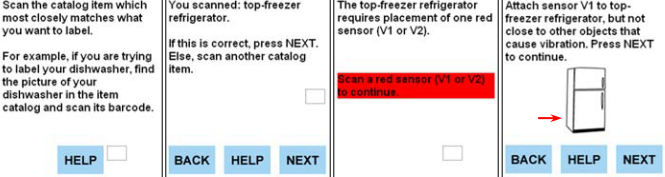
\includegraphics[width=0.8\textwidth]{img/assembly-doku_c.png}
  \caption{Bild des Kits}
  \label{fig:assembly-doku_c}
\end{figure}

Die Installation von Sensoren wird in \cite{Beckmann2004} als eine
Aufgabe mit zwei Dimensionen betrachtet: Platzierung und Assoziation.
Dies sind wichtige Anhaltspunkte um die Randbedinugnen des Modells zu
definieren.


%============================
Expertenwissen wird bei jeder generierung von Dokumentation ben�tigt.
Disadv: AR Handbook not linked to system model

Die Vorteile:
Sehr intuitiv
Automatisch erlernte Dokumentation der Schritte
Unterst�tzung bei der Verifikation der Arbeitsschritte
Passt die Videoausgabe an den Nutzer an

Probleme:
M�ssen wenigstens ein mal Aufgezeichnet werden
F�r Systeme mit vielen Varianten ein potenzielles Problem
�nderung der Prozessschritte zieht ein neues Durchspielen nach sich
Mit Software GUIs nicht ausprobiert
Noch keine Nutzbarkeitsstudie
Expertenwissen wird bei jeder generierung von Dokumentation ben�tigt.
Disadv: AR Handbook not linked to system model

Textuelle Handb�cher genau so gut oder besser?
